\section{The $\lambda$ Calculus}

\subsection{The Untyped $\lambda$-Calculus}
A evolução de universos não tipados para universos tipados pode ser ilustrada pelo cálculo $\lambda$, inicialmente desenvolvido como uma notação não tipada para capturar a essência da aplicação funcional de operadores a operandos.
As expressões no cálculo $\lambda$ têm a seguinte sintaxe\footnote{Usamos diversão em vez do $\lambda$ tradicional para trazer à tona a correspondência com as notações da linguagem de programação}:
\begin{figure}[h]
    \centering % para centralizarmos a figura
    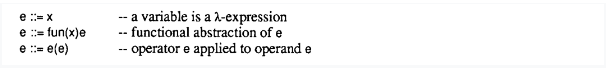
\includegraphics[]{anexos/Screenshot_40.png}
\end{figure}
\par A função de identidade e a função sucessora podem ser especificadas no cálculo $\lambda$ como a seguir.
Usamos o valor da palavra-chave para introduzir um novo nome vinculado a um valor ou função:
\begin{figure}[h]
    \centering % para centralizarmos a figura
    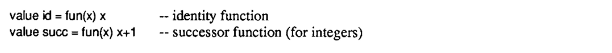
\includegraphics[]{anexos/Screenshot_39.png}
\end{figure}

\subsection{The Typed $\lambda$-Calculus}
O cálculo $\lambda$ digitado é como o cálculo $\lambda$, exceto que cada variável deve ser explicitamente digitada quando introduzida como uma variável limitada.
Assim, a função sucessora no cálculo $\lambda$ digitado tem a seguinte forma:
\pagebreak
\begin{figure}[h]
    \centering % para centralizarmos a figura
    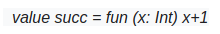
\includegraphics[]{anexos/Screenshot_41.png}
\end{figure}
\subsection{Basic Types, Structured Types, and Recursion}
O cálculo $\lambda$ digitado é geralmente acrescido de vários tipos básicos e estruturados, os quais usaremos:

\begin{figure}[h]
    \centering % para centralizarmos a figura
    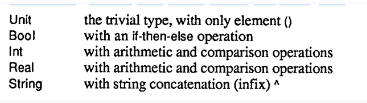
\includegraphics[]{anexos/Screenshot_42.png}
\end{figure}

\par Tipos estruturados podem ser construídos a partir desses tipos básicos por meio de construtores de tipo.
Os construtores de tipo em nossa linguagem incluem espaços de função ($\rightarrow$), produtos cartesianos ($x$), tipos de registro (também chamados de produtos cartesianos rotulados) e tipos de variantes (também chamados de somas disjuntas rotuladas).